\documentclass[acmtog]{acmart}
\usepackage{ctex}
\usepackage{graphicx}
\usepackage{subfigure}
\usepackage{natbib}
\usepackage{listings}
\usepackage{bm}
\usepackage{amsmath}
\usepackage{amssymb}
\usepackage{float}
\usepackage{subfigure}

\definecolor{blve}{rgb}{0.3372549 , 0.61176471, 0.83921569}
\definecolor{gr33n}{rgb}{0.29019608, 0.7372549, 0.64705882}
\makeatletter
\lst@InstallKeywords k{class}{classstyle}\slshape{classstyle}{}ld
\makeatother
\lstset{language=C++,
	basicstyle=\ttfamily,
	keywordstyle=\color{blve}\ttfamily,
	stringstyle=\color{red}\ttfamily,
	commentstyle=\color{magenta}\ttfamily,
	morecomment=[l][\color{magenta}]{\#},
	classstyle = \bfseries\color{gr33n}, 
	tabsize=1
}
\lstset{basicstyle=\ttfamily}

% Title portion
\title{Assignment 1:\\ {Exploring OpenGL and Phong Lighting}} 

\author{Name:\quad 王鹏豪  \\ student number:\ 2021533138
\\email:\quad wangph1@shanghaitech.edu.cn}
\setlength{\headheight}{25pt}
% Document starts
\begin{document}
\maketitle

\vspace*{2 ex}

\section{Introduction}
\begin{itemize}
	\item Task 1:\quad Load Mesh from File has been down
	\item Task 2:\quad Phong Lighting has been down
	\item Task 3:\quad Camera Control has been down
	\item Bonus1:\quad Play With Light has been down
	\item Bonus2:\quad Geometry Shader has been down
\end{itemize}
\section{Implementation Details}
\subsection{Load Mesh From File}
	In this section, we need to load mesh and draw it onto the screen.
\subsubsection{Load Part}
	In this section, we need to load mesh of .obj format, the .obj file is consist of three parts:
	\begin{itemize}
		\item \emph{v} is the position of vertices of 3 floats
		\item \emph{n} is the normal vector of vertices of 3 floats
		\item \emph{f} is the indices of each face of 6 ints
	\end{itemize}
	As for \emph{v}, we can directly push it into \emph{vertices} as \emph{Vertex} of \emph{position}.
	As for \emph{n}, because we haven't known the corresponding relationship with \emph{v},
	we can store it in a \emph{temp} vector.
	As for \emph{f}, we need first store the indices of \emph{Vertex} into \emph{indices},
	then as we have the corresponding
	relationship of \emph{v} and \emph{n}, we need to push the normal
	stored in \emph{tmep} vector into corresponding \emph{Vertex} of \emph{normal}. 
\subsubsection{Draw Part}
	In this section, we need to draw the loaded mesh to the screen. First we need to define:
	\begin{itemize}
		\item VAO Vertex Array Object
		\item VBO Vertex Buffer Object
		\item EBO Element Buffer Object
	\end{itemize}
	then make corresponding binding, then we use \textbf{glDrawElements()} and pass \emph{indices.size()} to it
	to draw all the triangles of the mesh.
	Meanwhile, vertexshader and fragment shader is also needed to draw the mesh correctly. 
	\begin{itemize}
		\item vertexshader	\par we need to define it as a single file like \emph{vertexshader.glsl}
			first we set aPos of vertex location and aNormal of vertex Normal to attribute location 0,1
			then as mesh is 3D model, we need matrix to transform the vertices location, so we define three uniform matrix
			\emph{model}, \emph{view}, \emph{proj}, 
			\begin{itemize}
				\item \emph{model} matrix includes shifting, scaling, rotating transforms
				\item \emph{view} matrix is used to move the scene to make it visible
				\item \emph{proj} matrix has 2 types: \emph{Orthographic Projection Matrix} and \emph{Perspective Projection Matrix}
					, it is used to transform coordinate from \textbf{view space} to \textbf{clip space}.
			\end{itemize}
			First our model vertex location coordinate is located at \textbf{local space}, we use \emph{model} matrix to transform it
			into \textbf{world space}, 
			Second as all the output pictures is viewed from a specific location of camera, we need \emph{view} matrix to transform
			the coordinate into \textbf{view space}.
			Third we needed to transform the coordinate into \textbf{clip space}, where vertex out of a specific frustum
			should be clipped. We needed to use \emph{proj} matrix.
			Fourth we needed to perform a viewport transform to transform it into screen space. 
			Lastly we needed to combine these matrix together, we have \(V_{clip} = M_{projection} \cdot M_{view} \cdot M_{model} \cdot V_{local}\)

		\item fragementshader \par we need to define it as a single file like \emph{fragementshader.glsl}
			as no light is demanded, we can directly output the color as an constant.
	\end{itemize}
\subsection{Phong Lighting}
	In this section we needed to implment three types of lighting and add them together
	\begin{itemize}
		\item Ambient Lighting, even there is no lighting, we also has light in the environment,
			we could simply set a constant of ambient strength and multiply it with object color.
		\item Diffuse Lighting, to calculate this lighting, we need normal and direct lighting.
			we already have the normal stored in the \textbf{Vertex.normal}, 
			then we needed to get the direct light, we need the position of light and fragment
			which is \textbf{lightpos} and \textbf{FragPos}, then we make a minus of them to get
			direct light which is \textbf{lightDir}, then make a dot operation of \textbf{norm} and \textbf{lightDir},
			then muptiply it with light color.
		\item Specular Lighting, this comes from the reflection of light on the surface of objects,
			we needed the viewer's position which is the camera's position. Then make a minus of \textbf{viewPos} and \textbf{FragPos},
			and because of the reflection, we need reflect function to reflect it.
			Then make a dot operation with \textbf{viewDir} and \textbf{reflectDir}, and make a pow operation.
			The power exponent, is just the shininess.
	\end{itemize}
\subsection{Camera Control}
	In this section, we need to response to keyboard's input and mouse's input.
	\subsubsection{keyboard input}
		In this section, we process keyboard input. Keyboard will infect the camera's position,
		to deal with this, we need to define three vector of the camera. Up, Forward, Right vectors.
		We need to mapping WASD to Forward and Right vectors' add or minus. I also mapping Space and C
		to Up vector to make the camera able to move in three axis.
	\subsubsection{mouse input}
		In this section, we process mouse input. Mouse input includes horizontal mouse movement affects the yaw and vertical mouse movement affects the pitch.
		We need tell GLFW to hide cursor and capture the mouse input. After define callback functions, we need to register them.
		We need to calculate the offset perframe and add or minus them to pitch. Also, a restrict need to add to the operation.
\subsection{Bonus 1} 
	In this section, I try to add a flashlight to the scene. First the same with point light, it contains
	ambient, diffuse, specular lights. As for flashlight, it is bright in the center, and dark if out of a specific area.
	We always want a little light even out of range, so the ambient will not be effected. We define a intensity
	and multiply diffuse and specular with it. The representition of I is \(I = \frac{\theta - \gamma}{\epsilon}\)
	$\epsilon$ is the cosine difference between the inner $\phi$ and the outer cone $\gamma$
	that is to say \(\epsilon = \phi - \gamma\). The $\theta$ is used to decide if the object is in the flashlight's inner area.
\subsection{Bonus 2}
	In this section, we need to add fur to model, first we can make normal visible, that is, add a set of vs, gs, fs.
	where using gs to make line to present normal. First use vs to get normal vector,
	then in gs, we make a line of one endpoint is on the surface of the triangles, another one is the point add the normal vector.
	We get a line, and then simply draw it out using gs.
\section{Results}
% pictures should be in
\begin{figure}[H]
	\centering
	\subfigure[basic]{
		\label{base_part}
		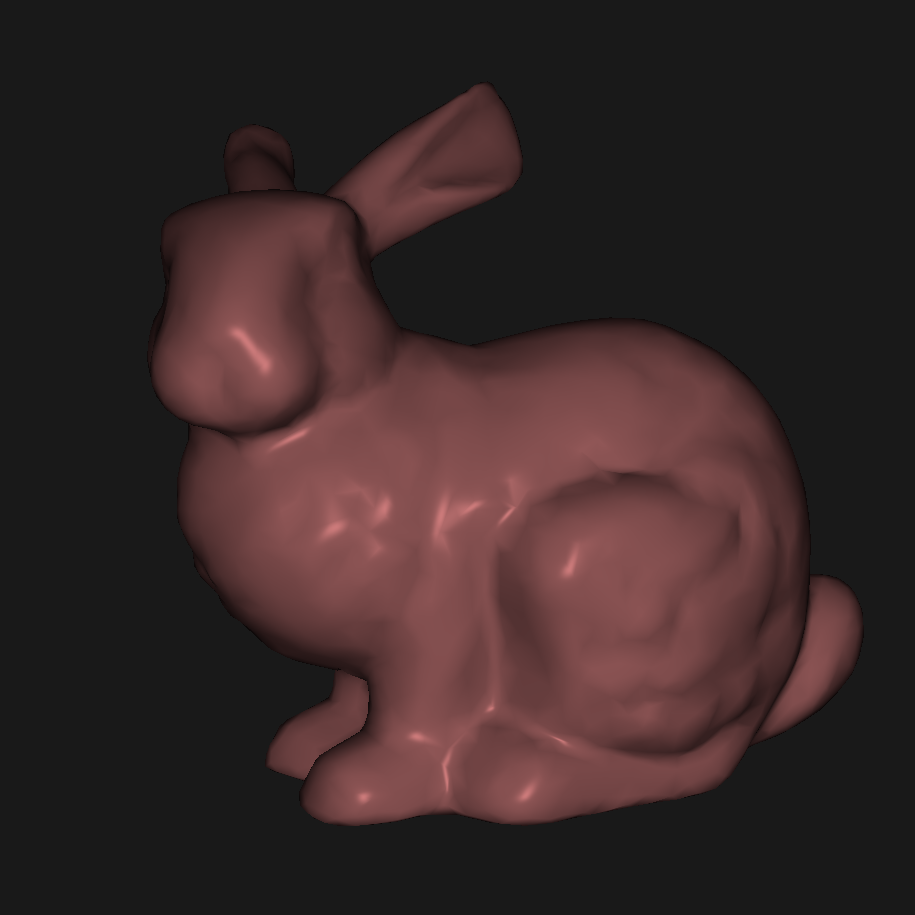
\includegraphics[width=0.2\textwidth]{base_part.png}}
	\subfigure[bonus1]{
		\label{bonus1}
		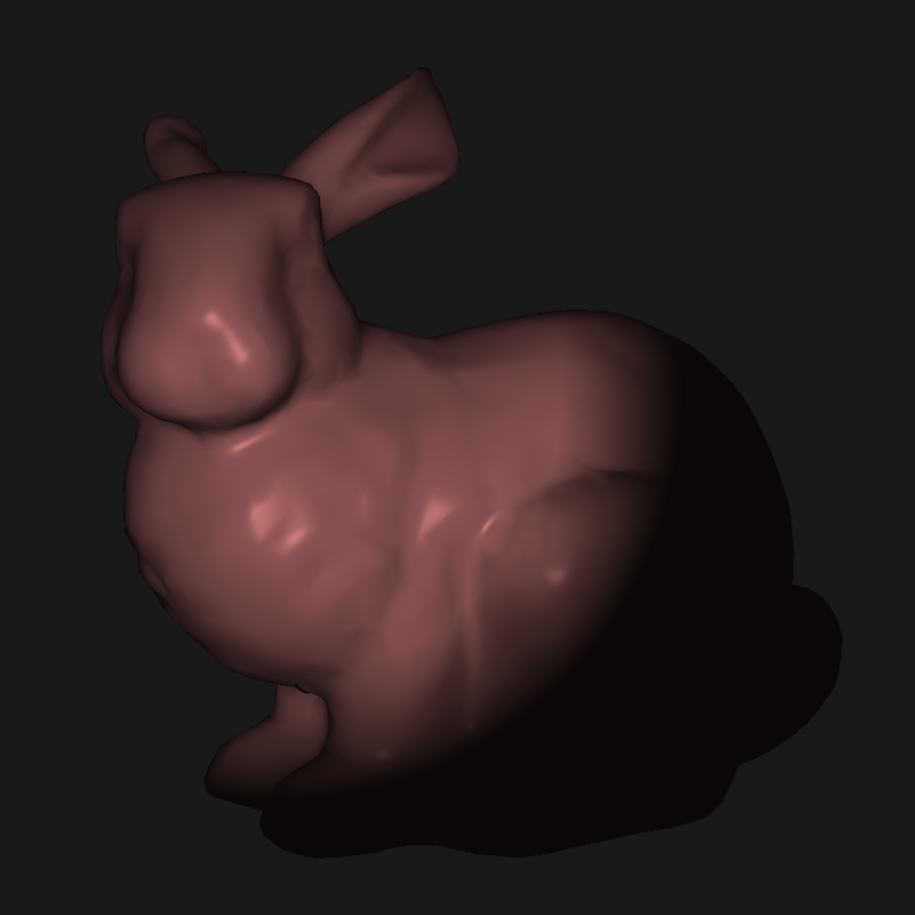
\includegraphics[width=0.2\textwidth]{bonus1.png}}
	\subfigure[bonus2]{
		\label{bonus2}
		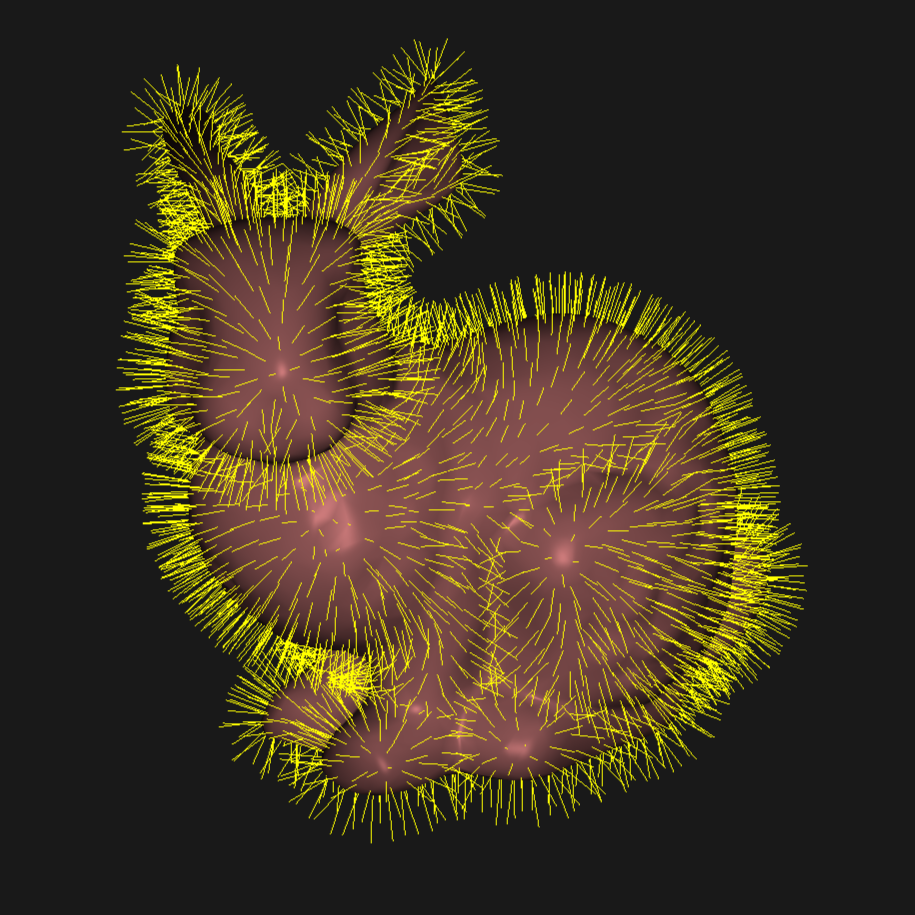
\includegraphics[width=0.2\textwidth]{bonus2.png}}
	\caption{Results}
	\label{Fig.main}
	\end{figure}
\end{document}
